\begin{question}
\noindent In a Valorant tournament, the map designer represents the positions of two objective markers, triangle $A$, on a coordinate grid. Triangle $A$ is translated by the vector $\begin{pmatrix} 4 \\ -5 \end{pmatrix}$ to give triangle $B$.

\begin{center}
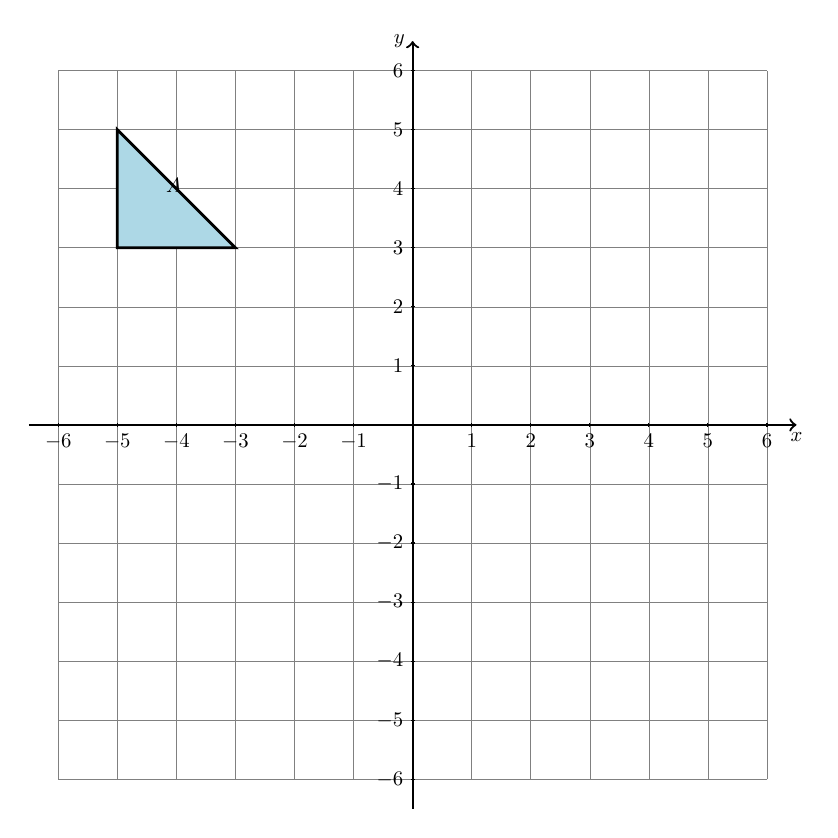
\begin{tikzpicture}[scale=0.75, transform shape]
    \definecolor{borderColour}{HTML}{000000}
    \definecolor{fillColourA}{HTML}{ADD8E6}

    \def\axisLimit{6}

    % Draw grid
    \draw[step=1cm,gray,very thin] (-\axisLimit,-\axisLimit) grid (\axisLimit,\axisLimit);

    % Draw axes
    \draw[thick,->] (-\axisLimit-0.5,0) -- (\axisLimit+0.5,0) node[anchor=north] {$x$};
    \draw[thick,->] (0,-\axisLimit-0.5) -- (0,\axisLimit+0.5) node[anchor=east] {$y$};

    % Label x-axis and y-axis
    \foreach \x in {-\axisLimit,...,-1,1,2,...,\axisLimit}
        \draw (\x cm,1pt) -- (\x cm,-1pt) node[anchor=north] {$\x$};
    \foreach \y in {-\axisLimit,...,-1,1,2,...,\axisLimit}
        \draw (1pt,\y cm) -- (-1pt,\y cm) node[anchor=east] {$\y$};

    % Define vertices of triangle A
    \coordinate (P) at (-5,3);
    \coordinate (Q) at (-5,5);
    \coordinate (R) at (-3,3);

    % Draw triangle A
    \filldraw[fill=fillColourA, draw=borderColour, line width=1pt] (P) -- (Q) -- (R) -- cycle;
    \node[below right] at (-4.3,4.3) {$A$};

\end{tikzpicture}
\end{center}

\noindent On the grid, draw triangle $B$, the image of triangle $A$ after this translation.

\vspace{4cm}

\begin{flushright}
    \answermarks{2}
\end{flushright}
\end{question}
